\documentclass[tikz, border=50pt]{standalone}

\usepackage{graphicx}
\usepackage{color}
\usepackage{tikz}
\usepackage{geometry}

\usetikzlibrary{calc}

% Use sans everywhere, first line for sans text and second two for sans math
\renewcommand{\familydefault}{\sfdefault}
\usepackage{sansmath}
\sansmath           

\usetikzlibrary{arrows.meta,calc,positioning,shapes.arrows,3d}
\graphicspath{ {./images/} } 

\begin{document}

	%\noindent\resizebox{\textwidth}{!}{
	\begin{tikzpicture}[
	Arrow/.style = {single arrow,draw,
    minimum height=8mm, 
    minimum width=2mm,
    rotate=0}]
    % can also specify z axis slope eg [scale=.8, z={(-.707,-.3)}]
	%\draw[use as bounding box, transparent] (-1.8,-1.8) rectangle (17.2, 3.2);

		\newcommand{\networkLayer}[5]{
			\def\q{0.02} %parameter for filling			
			
			\def\s{#1} % Size of square			
			\def\x{#2} % X distance 
			\def\y{#3} % Y distance 
			\def\z{#4} % Z distance 

			% NOTE: X axis passes through centre of default square (if Y and Z are both zero) 
			% Construct clockwise from bottom back 
			\coordinate (A) at (\x,-\s/2+\q/2+\y,-\s/2+\q+\z); 
			\coordinate (B) at (\x,-\s/2+\q/2+\y,\s/2-\q+\z);
			\coordinate (C) at (\x,\s/2-\q/2+\y,\s/2-\q+\z);
			\coordinate (D) at (\x,\s/2-\q/2+\y,-\s/2+\q+\z);

			\filldraw[#5] (A) -- (B) -- (C) -- (D);  % Fill before draw edges

			\draw[line width=0.3mm] (A) -- (B);  % Bottom line
			\draw[line width=0.3mm] (B) -- (C);  % Vertical front
			\draw[line width=0.3mm] (C) -- (D);  % Top line
			\draw[line width=0.3mm] (D) -- (A);  % Vertical back

		}
		
		\newcommand{\pyramid}[6]{
			\def\q{0.02} %parameter for filling			
			
			\def\s{#1} % Size of square			
			\def\x{#2} % X distance 
			\def\y{#3} % Y distance 
			\def\z{#4} % Z distance

			% NOTE: X axis passes through centre of default square (if Y and Z are both zero) 
			% Construct clockwise from bottom back 
			\coordinate (A) at (\x,-\s/2+\q/2+\y,-\s/2+\q+\z); 
			\coordinate (B) at (\x,-\s/2+\q/2+\y,\s/2-\q+\z);
			\coordinate (C) at (\x,\s/2-\q/2+\y,\s/2-\q+\z);
			\coordinate (D) at (\x,\s/2-\q/2+\y,-\s/2+\q+\z);

			% Use 'fill=none' if needed
			\filldraw[#5] (A) -- (B) -- (C) -- (D);  % Fill before draw edges

			\draw[line width=0.2mm, color=gray!80] (A) -- (B);  % Bottom line
			\draw[line width=0.2mm, color=gray!80] (B) -- (C);  % Vertical front
			\draw[line width=0.2mm, color=gray!80] (C) -- (D);  % Top line
			\draw[line width=0.2mm, color=gray!80] (D) -- (A);  % Vertical back
			
			\def\d{#6} % Distance to point of pyramid
			\coordinate (E) at (\x+\d,\y,\z);
			\draw[line width=0.2mm, color=gray!80] (A) -- (E);  % 
			\draw[line width=0.2mm, color=gray!80] (B) -- (E);  % 
			\draw[line width=0.2mm, color=gray!80] (C) -- (E);  % 
			\draw[line width=0.2mm, color=gray!80] (D) -- (E);  % 

		}
		
		

%%%%%%%%%%%%%%%%%%%%%%%%%%%%%%%%%%%%%%%%%%%%%%%%%%%%%%%%%%%%
%%%%%%%%%%%%%%%%%%%%%%%%%%%%%%%%%%%%%%%%%%%%%%%%%%%%%%%%%%%%
%%%%%%%%%%%%%%%%%%%%%%%%%%%%%%%%%%%%%%%%%%%%%%%%%%%%%%%%%%%%

		% INPUT
		% \networkLayer{6.0}{0}{0}{0}{color=gray!80};
		\node[canvas is zy plane at x=0,draw,fill=white] at (0,0) {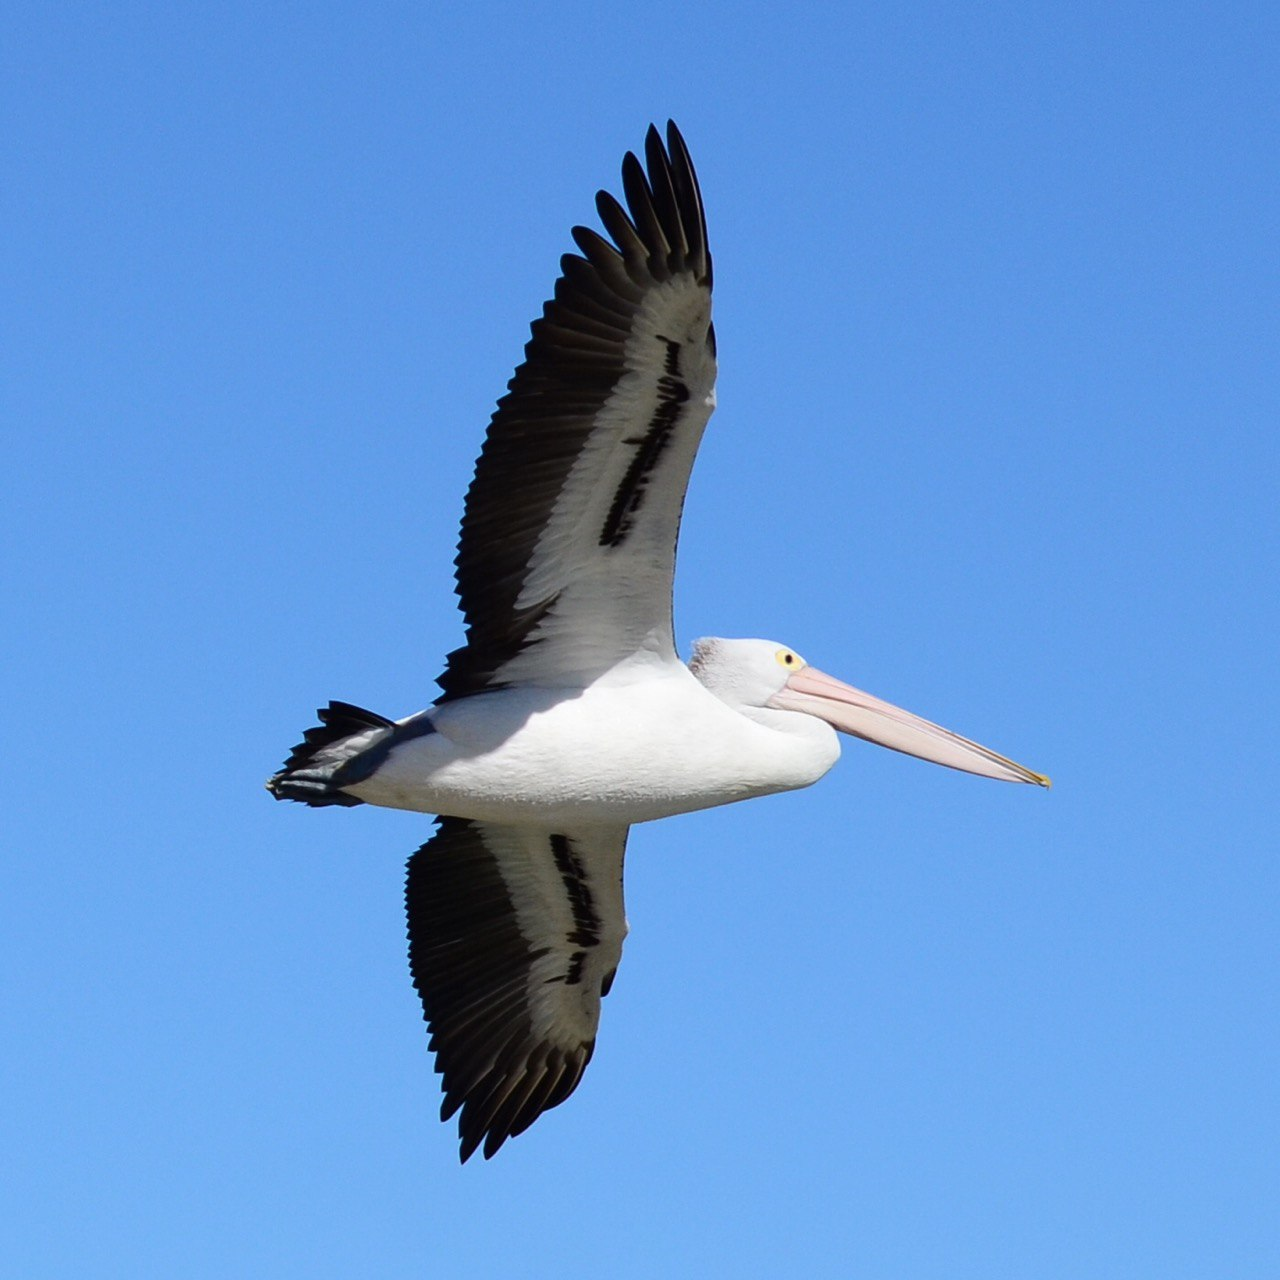
\includegraphics[scale=.14]{images/bird.jpeg}};
		
		\pyramid{1.28}{0}{1.79}{1.43}{color=blue!50, opacity=0.5}{4};

		% First convolutional layer
 		\foreach \i in {0,...,5} 
   			\networkLayer{5}{4+\i*2/10}{0}{0}{color=white};   	

		\pyramid{0.5}{5.4}{1}{1}{color=gray!10}{3};  % Last arument is depth to point

		
		% First maxpool layer
 		\foreach \i in {0,...,7} 
   			\networkLayer{3}{8.4+\i*2/10}{0}{0}{color=white}; 

		\pyramid{0.8}{9.8}{1}{0.8}{color=gray!10}{3};  


		% Second convolutional layer
 		\foreach \i in {0,...,11} 
   			\networkLayer{2.5}{12.8+\i*2/10}{0}{0}{color=white};  

		\pyramid{0.5}{15.3}{1}{1.2}{color=gray!10}{3}; 	

		% Second maxpool layer
 		\foreach \i in {0,...,15} 
   			\networkLayer{1.5}{17.8+\i*2/10}{0}{0}{color=white};   

		\coordinate (A1) at (22.8,-3,0) ; 
		\coordinate (A2) at (22.8,3,0) ; 		
		\coordinate (B1) at (24.8,-1,0) ; 
		\coordinate (B2) at (24.8,1,0) ; 		
		\coordinate (C1) at (26.8,-1,0) ; 
		\coordinate (C2) at (26.8,1,0) ; 
		\coordinate (A11) at (20.5,-1,0) ; 
		\coordinate (A12) at (20.5,0.45,0) ; 

		% Reshape
		\draw[line width=1mm] (A1) -- (A2);
		\draw[line width=0.1mm] (A) -- (A1);  	
		\draw[line width=0.1mm] (D) -- (A2);  

		% Fully connected Dense (dim of 10!)
		\draw[line width=1mm] (B1) -- (B2); 
		\draw[line width=0.1mm] (A1) -- (A11); 
		\draw[line width=0.1mm] (A2) -- (A12);
		\draw[line width=0.1mm] (A1) -- (B1);
		\draw[line width=0.1mm] (A1) -- (B2);		  	
		\draw[line width=0.1mm] (A2) -- (B1);
		\draw[line width=0.1mm] (A2) -- (B2);

   		\node[Arrow]  at (25.8,0,0) {};

	   	\node[text width=3cm,align=center]  at (26.8,0,0) {$Bird$};
	
	\end{tikzpicture}
	%}

\end{document}
